\documentclass[../main.tex]{subfiles}
\graphicspath{{resources/}{resources/mbed_res}}

\begin{document}

\section{Beágyazott szoftver elkészítése}
    %\subsection{Beágyazott szoftver}
        A beágyazott szoftver feladata, hogy a Wifi modultól érkező csomagokat fogadja, értelmezze, majd ez alapján meghatározza és kiküldje a LED sor által értelmezhető formátumban a jeleket. A feladatot erre a mikrokontrollerre három féle könyvtárcsomaggal is meg lehet oldani. 
        
        \begin{itemize}
            \item Arduino környezettel
            \item HAL (Hardware Abstraction Layer) könyvtárral
            \item SPL (Standard Peripherals Library) könyvtárral
        \end{itemize}
        
        Az Arduino környezetben már rengeteg megoldás létezik az interneten az ilyen típusú LED sorok vezérlesére. Az egyiket kiválasztva, letöltve és kisebb módosításokat végezve a programkódon a Wifi modullal való kommunikáció is megoldható. Ez a módszer már elsőre is jól hangzik, de projekt célja nem a gyors működésre bírás, hanem a háttérben futó folyamatok megértése, és az Arduino-s megoldás pont ezt rejti el. Hasonló megoldást kínál az ST gyártó a HAL könyvtárakkal. A már használt STM32CubeMX programban a megfelelő IDE-be (Integrated Development Environment - integrált fejlesztői környezet) lehet generálni majdnem kész projekteket. Egy pár kattintással be lehetne állítani az órajel konfigurációt, az I/O portok, időzítők (továbbiakban Timer), megszakítók (továbbiakban Interrupt), stb. működését életünket jelentősen megkönnyítve. Viszont, mint ahogy a neve is súgallja, hardver absztrakciós réteg, ez a megoldás is elfedi a belső működését a mikrokontrollernek. Az igényeimet végeredményül az SPL könyvtár fogja kielégíteni, ami hozzáférést ad a regiszterekhez, de emellett alapszintű függvényeket is biztosít a folyamatok kezeléséhez. //TODO ref
        %hal spl
        %https://www.purplealienplanet.com/node/61
        %https://electronics.stackexchange.com/questions/225568/stm32f4-and-hal
        
        A perifériakezelést mindkét esetben DMA-val (direkt memória hozzáférés) valósítottam meg, hogy a processzor ez idő alatt mással tudjon foglalkozni. Az egyes részelemeket az átláthatóság kedvéért igyekeztem külön könyvtárakba csoportosítani, illetve az extra moduloknak további alkönyvtárakat létrehozni. 
        
        Az adott lábak, periféria, órajelek engedélyezésénél nagy segítségemre volt az adatlapban megtalálható mikrokontroller blokkvázlata (\ref{fig:stm32f103xx_block_diagram}. Ábra). A diagramm megmutatja, hogy melyik buszt, illetve mikor minek az órajeleit kell engedélyezni. Például, ha a SPI1-t szeretném használni, akkor nem csak SPI1 vezérlő számára kell biztosítani a működéshez szükséges órajelet, hanem az APB2 (Advanced Peripheral Bus 2) részére is engedélyezni kell.
        \begin{figure}[h!]
            \centering
                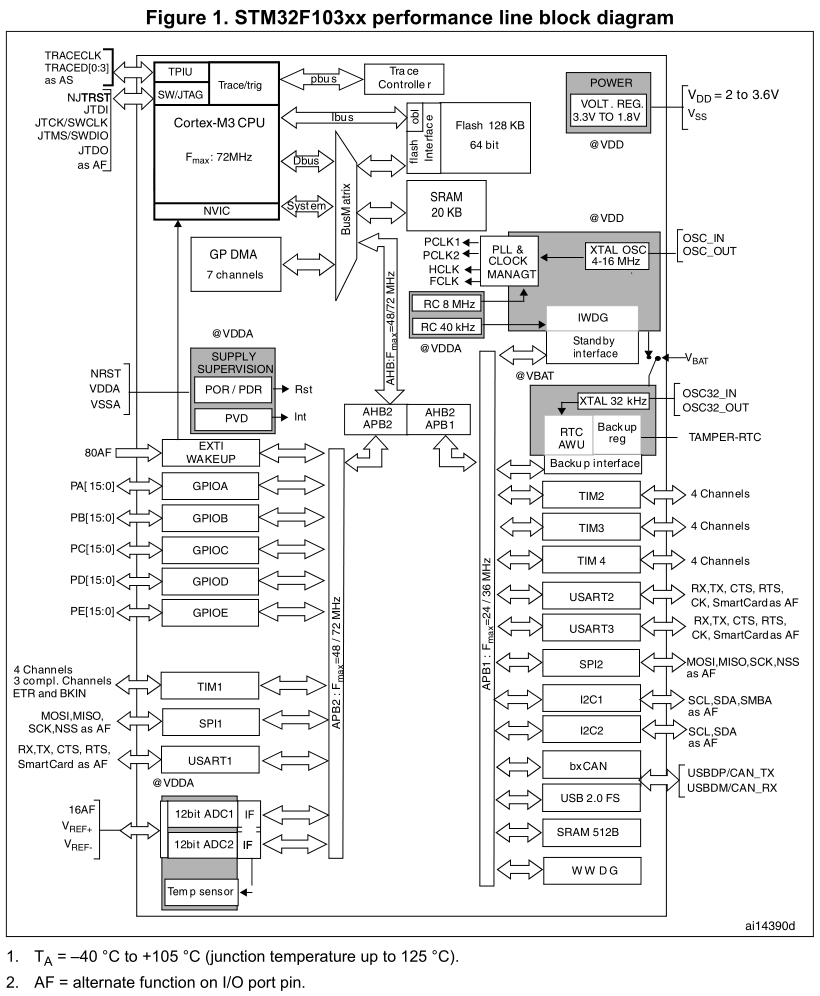
\includegraphics[width=10cm]{resources/mbed_res/stm32f103xx_block_diagram.png}
                \caption{STMF103XX blokk diagrammja}
                \label{fig:stm32f103xx_block_diagram}
        \end{figure}
        
        A beágyazott szoftver megírását négy részre bontottam le:
        \begin{enumerate}
            \item Mikrokontoller inicializálása
            \item LED sorral való kommunikáció (PWM)
            \item Wifi modullal való kommunikáció (UART)
            \item Az előző kettő összekötése
        \end{enumerate}
        
        A szakdolgozatomban nem fogok kitérni arra, hogy konkrétan melyik regiszterek, illetve milyen értékek lettek beállítva, hanem a lényegi összefüggéseket írom le.
    
    \subsection{STM32F103C8T6 mikrokontroller inicializálása}
        A mikrokontroller programozására és debuggolására az ST tulajdonában lévő, ingyenesen elérhető, cross platform Atollic TrueStudio-t használtam. Az IDE Eclipse alapú és rengeteg beágyazott szoftver fejlesztésében segítő eszközzel van kiegészítve. Az STM32CubeMX programban létrehozott projektünket egy az egybe lehet exportálni az IDE-be, persze ilyenkor HAL könyvtárakat használ a projekt.
        Új projekt készítésékor a régi mikrokontrollerekhez, viszont az SPL-t is lehet használni. A mikrokontroller és a debugger fajtája (JTAG/SWD), és még egy pár opció beállítása után egy azonnal fordítható kódot generál.
        A projektet lebuildelve és felflashelve a mikrokontrollerre, az a main.c állonmányt fogja futtatni, illetve az \textit{main()} függvény a program belépési pontja.
        
        \begin{figure}[h!]
            \centering
                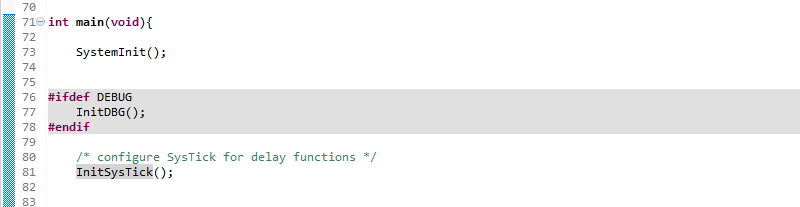
\includegraphics[width=13cm]{resources/mbed_res/ps_main_init.png}
                \caption{main.c állomány eleje}
                \label{fig:ps_main_init}
        \end{figure}
        
        A \textit{main()} függvény első soraiban (\ref{fig:ps_main_init}. Ábra) kell beállítani kívánt működési órajelet. Ezt a SPL egyik könyvtárában lévő \textit{SystemInit()} nevű függvény végzi el. A függvény alapértelmezett beállítása a 72MHz-es órajel, pont amit én is be akarok állítani. A következő sorokban a DEBUG szó definiálására lefutó \textit{InitDBG()} függvény (//TODO ref vass peter -github). Ebben a függvényben beállításra került, hogyha debuggolásnál megállítjuk a CPU futását, akkor a Timer-ek is megálljanak. Az inicializálást az \textit{InitSysTick()} függvény zárja, amiben be lett állítva hogy a \textit{SysTick_Handler()} interrupt kezelő függvény mikor hívódjon meg. Ez a függvényre épülnek a \textit{util} könyvtárban megtalálható primitív \textit{Delay..()} függvények, és a mikrokontroller helyes működését visszajelző LED villogtatásának.
       
    \subsection{LED sorral való kommunikáció}
     %   \subsubsection{LED sorral való kommunikáció}
        //TODO ref ws2811 datasheet
        Egy LED szalagot egy darab, egy irányú jelcsatornán lehet vezérelni. Ezen a vezetéken kivezérelt megfelelő frekvenciájú PWM (Pulse Width Modulation - impulzus szélesség moduláció) jel kitöltési tényezőjének változtatásával lehet a WS2811-es IC számára a megfelelő bitkombinációt elküldeni. 400kHz-es üzemmódban a '0'-s bithez egy 0,5\micro s ideig magas, és 2,0\micro s ideig alacsony, azaz 20\%-os kitöltési tényezőjű PWM ciklus felel meg. Az '1'-s bithez pedig egy 1,2\micro s ideig magas, és 1,3\micro s ideig alacsony, azaz 48\%-os kitöltési tényezőjű PWM ciklus felel meg. Egy IC számára egy RGB kódnak megfelelő 24bit szélességű adatot (24 darab PWM ciklus) kell elküldeni, 8-8-8 bites felbontással. Ezen felül érkező biteket továbbítja a következő - vele sorba kapcsolt - IC-nek. Az IC-k a kimenetére kötött LED-eken akkor fog megjelleni az elküldött szín, mikor egy reset jel érkezik. A reset jel egy 50\micro s-nál hosszab alacsony feszültség szint. A 800kHz-es üzemmódban az idők a reset jel kivételével a felére csökkennek. 
        Az általam vásárolt LED sorokon 50 darab ilyen WS2811-es IC található, IC-ként 3 darab RGB LED-del. Ezeket a LED-hármasokat neveztem el ledgroup-oknak (LED csoportoknak), mert ezeknek a színeit lehet külön-külön változtatni. 
        
        \subsubsection{PWM jel létrehozása a kimeneteken}
            A LED sor vezérlésére a hármas Timer (továbbiakban TIM3) 2,3,4-es csatornáit (továbiakkban CHx, ahol az 'x' jelenti az adott csatorna számát) használtam, mert ezek felelnek meg a kapcsolásban bekötött lábaknak (PA7,PB0,PB1). Első körben engedélyezni kell az I/O portokra (esetemben A és B portokra) és az AFIO-ra (alternate function I/O) az órajelet. Az utóbbira azért van szükség, mert a TIM3 ezen keresztül fogja vezérelni az mikrovezélrő lábait. A I/O portokon beállítottam a megfelelő lábakat kimenetre és hogy milyen sebességgel fognak maximálisan operálni.
            
            
            Második lépés a TIM3 működési frekvenciájának beállítása. A TIM3 az APB1-en található (\ref{fig:stm32f103xx_block_diagram}. ábra), de az összes többi periférával ellentétben az timerek megkapják a 72MHz-es órajelet (\ref{fig:tim3_clk_src}. ábra). Alapvetően a 800kHz-es módra konfiguráltam fel a TIM3-at, mert az előosztó (prescaler) megváltoztatásával 400kHzes működési mód érhető el.
            A legnagyobb felbontás elérése érdekében egyre választottam az órajelosztást, ami azt jelenti hogy 72MHz-en fog üzemelni a timer. Ezen a frekvencián 90 órajelciklus fel meg 1,25\micros-nak, a 800kHz-es jel periódusidejének. A TIM3 tehát 0-tól fog számolni 89-ig, ahol nullázódik és kezdi újra a számlálást. Azt hogy ez idő alatt mit csinál, az Output Compare mód beállításával lehet megadni.
            Az előosztót (prescaler) a LED sor könyvtárában való sebesség módok definiálásával változtathatóvá tettem (\ref{fig:ws2811_timing_values}. ábra). Eredményül a lassabb 400kHz mód esetén felére csökkenti a TIM3 működési frekvenciáját, ezzel a kívánt működést okozva.
            
            \begin{figure}[h!]
                \centering
                    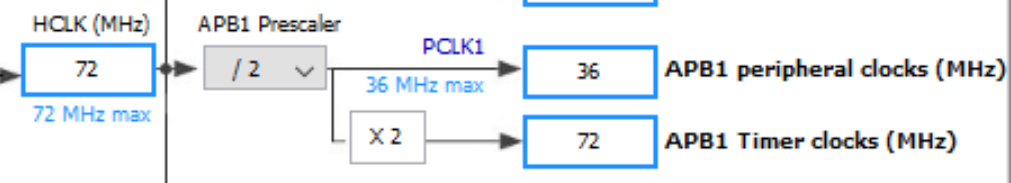
\includegraphics[width=10cm]{mbed_res/tim3_clock_src}
                \caption{APB1 órajelei az STM32CubeMX programból}
                \label{fig:tim3_clk_src}
            \end{figure}
            
            Harmadik lépés a működési mód és tulajdonságainak bekonfigurálása. Kimenetbe, azon belül a PWM1 üzemmódba állítottam a timert. Az alapértelmezett polaritás beállításoknál az annyit tesz, hogy mikor elkezd számlálni, akkor magas jelszintet ad ki, és mikor eléri a \textit{Capture Compare} (továbbiakban CC) értéket akkor vált alacsony (föld) jelszintre. A CC értékkel lehet majd beállítani, hogy milyen kitöltési tényezőnél történjen meg ez a váltás. 90 számlálásnál a logikai igaznak értelmezett 48\%-os kitöltési tényező 43-nak, míg a logikai hamis 20\%-os kitöltési tényező 18-nak fog megfelelni (\ref{fig:ws2811_timing_values}. ábra). A DMA vezérlés célja, hogy a CC értékét periódusonként változtassuk, ezzel a 24bit-es szín kombinációkat létrehozva a LED szalagon található WS2811 IC-k számára.
            
            \begin{figure}[h!]
                \centering
                    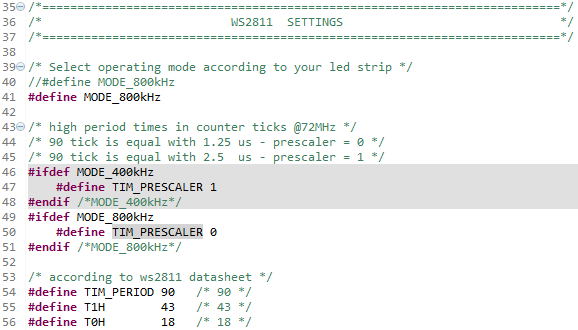
\includegraphics[width=12cm]{mbed_res/ws2811_timing_values}
                \caption{Képernyőkép a WS2811 nevű könyvtár header állományából}
                \label{fig:ws2811_timing_values}
            \end{figure}
         
        \subsubsection{PWM vezérlése DMA segítségével}  
             A beágyazott szoftverben egy tömben tárolom, hogy melyik LED sornak melyik ledgroupján milyen színt kell megjelenítsek. Ez a tömböt fogja majd később frissíteni a Wifi modulról érkező adat. Viszont a LED sor számára az egyes biteket, illetve a biteknek megfelelő kitöltési tényezőjű (CC értékű) PWM-et kell küldeni. Egy ledgroupnak 3 bájton tárolom a színét, viszont hogy ennek a három bájtnak, azaz 24 bitnek, a kitöltési tényezőjét eltároljam, 24 bájtra lenne szükségem (43, és 18 értékeket a legkisebb egységen, egy bájton lehet eltárolni). Szóval egy ledgroup kitöltési tényezőjének eltárolásához nyolcszor annyi hely szükséges, mint csak a színadataihoz. Ha 6 ledsort csatlakoztatnék az eszközömre akkor ($ 6[ledstrip]\cdot 50 [\frac{ledgroup}{ledstrip}] \cdot 3 [\frac{byte}{ledgroup}] = 900 [byte]$) 900 bájtot, és a kitöltési tényezőket még 7200 bájtot kellene eltároljak. Összesen tehát körülbelül 7,9 kilobájtot ($ (900+7200)/1024 \approx 7,9[kilobyte]$), ami a 64 kilobájtos tárhelynél már egeszén drasztikus. Ezért ezt valamilyen bufferezési technikával kell megoldanom.
             
             A reference manual timer regiszterei szekciót olvasva találtam rá az úgynevezett DMA Burst funkcióra. Ez a funkció lehetővé teszi, hogy a memóriában lévő tömbből az adatokat, ne csak egy, hanem több timer regiszterbe írja. A működés így a következőképpen készítettem el: az adatok írását a CH2 CC regiszterével kezdi és a CH4 regiszterrel fejezi be. 6 elemű adattömb esetén az 0-s indexú elem kerülne a CH2 CC regiszterébe, 1-es a CH3, 2-es a CH4, 4-es újra a CH2 CC regiszterébe, és így tovább. Tehát a buffer szerkezetemnek úgy kell kinéznie, hogy a párhuzamosan kapcsolt LED sorok azonos indexű bitjei legyen egymás után sorba rendezve.
             
             A DMA ciklikus üzemmódban is beállítható, így a memóriában található adatokon iterál végig, újból és újból. A DMA buffer méretét és a ledgroupok számának ismeretében meghatároztam hogy hány ciklus után kell lekapcsolni a DMA-t. Már csak a buffer megfelelő frissítését kell megoldanom a működéshez. A DMA vezérlőn be lehet kapcsolni a HT (half transfer - fél transzfer) és FT (full transzfer - teljes transzfer) interruptokat, amik jelzik, hogy a vezérlő végzett a fél, illetve egész buffer kiküldésével. Amikor megjelenik a HT interrrupt akkor fogom a buffer első felét frissíteni a következő adatokkal, a FT interruptnál pedig a buffer második felét. 
             
             A LED sort frissítése tehát a következő pontokra bomlik le, amit a \textit{refreshLedStrip()} függvényhívással (\ref{fig:ws2811_refreshledstrip}. ábra) indíthatunk el:
            \begin{enumerate}
                \item A ledgroup színeinek alapján a kitöltési tényezők meghatározása, és a bufferbe való betöltése
                \item A DMA vezérlő állapotának resetelése, buffer méretének a beállítása
                \item TIM3 elindítása
                \item A buffer frissítése a DMA megszakításkezelőjében
                \item Az adatok kiküldése után a TIM3 leállítása és várakozás legalább a 50\micros resetjel teljesüléséig
            \end{enumerate}
            
            \begin{figure}[h!]
                \centering
                    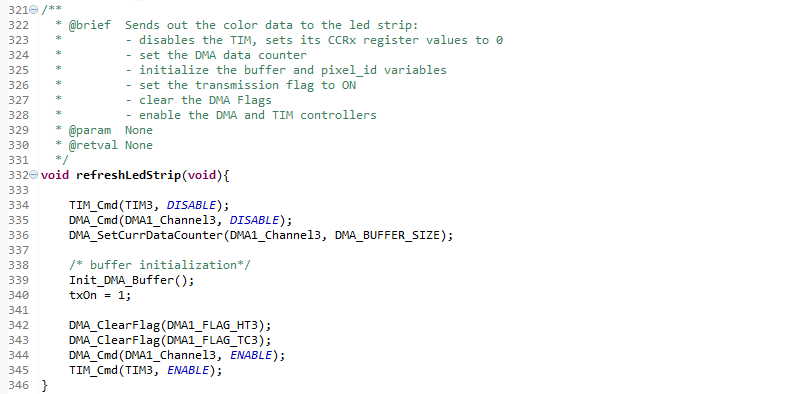
\includegraphics[width=12cm]{mbed_res/ws2811_refreshLedStrip}
                \caption{Képernyőkép \textit{refreshLedStrip()} függvényről}
                \label{fig:ws2811_refreshledstrip}
            \end{figure}
            
    \subsection{ESP8266-os Wifi Modul}
        
        
        
        
        
        
        kommunikalas az espvel - bekonfiguralasa
        adatszerkezet        
        effektek arduino neopixel librarybol

\end{document}